\section{Moment Closure Problem Revisited}
\label{sec:moment_problem_revisited}

In section~\ref{sec:moment_closure}, it was established that a choice for the second moment of the radiance distribution was required to close the system of equations, which was found by collapsing the moment expansion of the radiative transfer equation truncated after the first moment. The classical diffusion approximation was derived by assuming an isotropic radiance distribution for the second moment. In this section, we take a closer look at the moments and carve out an important feature, which explains the inaccuracy of classical diffusion approximation in certain scenarios.

The distribution of power $\phi$ over solid angle was given by the normalized radiance $\widehat{L}$. Since it is a probability distribution, it has to integrate to one, which is verified by
\begin{align*}
\int_{\Omega}{\hat{L}(\vec{x}, \vec{\omega})\ud\vec{\omega}}=
\int_{\Omega}{\frac{L\left(\vec{x}, \vec{\omega}\right)}{\phi\left(\vec{x}\right)}\ud\vec{\omega}}=
\frac{1}{\phi\left(\vec{x}\right)}
\int_{\Omega}{L\left(\vec{x}, \vec{\omega}\right)\ud\vec{\omega}}
=1
=\hat{L}_0
\end{align*}
Further, the normalized radiance $\widehat{L}$ has to be non-negative to be a probability distribution:
\begin{align*}
\hat{L}(\vec{x}, \vec{\omega})\ge 0 \qquad \text{for all unit directions } \vec{\omega}
\ ,
\end{align*}
which is verified by the fact, that the radiance field is non-negative by definition:
\begin{align*}
L\left(\vec{x}, \vec{\omega}\right) \ge 0
\implies
\int_{\Omega}{L(\vec{x}, \vec{\omega})\ud\vec{\omega}}=\phi\left(\vec{x}\right)\ge 0
\implies
\frac{L\left(\vec{x}, \vec{\omega}\right)}{\phi\left(\vec{x}\right)}=\widehat{L}(\vec{x}, \vec{\omega}) \ge 0
\end{align*}

Akhiezer~\cite{Akhiezer65} established, that the probability distribution contraints on a function results in a set of inequalities between moments of this function. In particular, the non-negativity constraint on the radiance field $L$ and its normalized distribution impose a constraint between the zero moment and the first moment. In case of the radiance field, this constraint can be derived by considering the dot product between direction vectors $\vec{\omega}'$ and $\vec{\omega}$, both of unit length. This results in the equation:
\begin{align*}
-1 \le \vec{\omega}'\cdot\vec{\omega} \le 1
\implies
0 \le 1 - \vec{\omega}'\cdot\vec{\omega} \le 1
\implies
\int_{\Omega}{\left(1-\vec{\omega}'\cdot\vec{\omega}\right)L\left(\vec{x}, \vec{\omega}\right)\ud\vec{\omega}}\ge 0
\end{align*}
which can be rearranged into:
\begin{align*}
\int_{\Omega}{\left(1-\vec{\omega}'\cdot\vec{\omega}\right)L\left(\vec{x}, \vec{\omega}\right)\ud\vec{\omega}} &\ge 0
\Leftrightarrow
\\
\int_{\Omega}{L\left(\vec{x}, \vec{\omega}\right)\ud\vec{\omega}}
-\int_{\Omega}{\vec{\omega}'\cdot\vec{\omega} L\left(\vec{x}, \vec{\omega}\right)\ud\vec{\omega}}
&\ge 0
\Leftrightarrow
\\
\int_{\Omega}{L\left(\vec{x}, \vec{\omega}\right)\ud\vec{\omega}}
-\vec{\omega}'\cdot\int_{\Omega}{L\left(\vec{x}, \vec{\omega}\right)\vec{\omega}\ud\vec{\omega}}
&\ge 0
\Leftrightarrow
\\
\phi\left(\vec{x}\right)
-\norm{\vec{E}\left(\vec{x}\right)}
&\ge 0
\Leftrightarrow
\\
\phi\left(\vec{x}\right)
&\ge \norm{\vec{E}\left(\vec{x}\right)}
\end{align*}
This constraint states, that the total power at position $\vec{x}$ must never exceed the length of the flux-vector. Considering that the flux-vector is found by integrating the radiance field over solid angle multiplied by a weighting factor between $\left[-1, 1\right]$ (the direction vector component). This must never be larger than the fluence, which is the integral over the radiance field itsself.

A very similar constraint can be derived for the normalized radiance $\widehat{L}$, by following the steps above. This results in:
\begin{align}
\label{eq:fld_flux_limit}
1
\ge
\norm{
\frac{\vec{E}\left(\vec{x}\right)}{\phi\left(\vec{x}\right)}
}
\end{align}
In the case of the classical diffusion approximation $\vec{E}\approx-D\nabla\phi$ (equation~\ref{eq:diffusion_ficks_law}). Inserting this into equation~\ref{eq:fld_flux_limit} gives:
\begin{align}
\label{eq:fld_flux_limit}
1
\ge
\norm{
\frac{\nabla\phi\left(\vec{x}\right)}{3\sigma_t\left(\vec{x}\right)\phi\left(\vec{x}\right)}
}
\end{align}
It shows, that with the classical diffusion approximation, this constraint can be violated when the extinction coeffient $\sigma_t$ becomes very small, meaning in the presence of very thin medium. It breaks down completely in case of vacuum $\sigma_t=0$. The constraint can also be violated if the the fluence gradient becomes very large in relation to $\sigma_t\phi$. This happens very close to point light sources and near strong density gradients in the medium.

Violation of the constraint above means, that for the classical diffusion approximation, the flux vector is much larger than what is physically possible. Since the flux vector governs light transport with diffusion, the literature often refers to classical diffusion as to suffer from unphysical fluxes or unphysical light transport.


\subsubsection*{A Transport Regime Measure}

The right hand side of equation~\ref{eq:fld_flux_limit} is an important measure, which allows to detect at every point within the domain, where and to what extend the diffusion approximation fails. For this only local information about the moments and extinction coefficient is needed. It is an important building block for the technique presented in this chapter, which seeks to improve the accuracy of the diffusion approximation.

The flux-limit in equation~\ref{eq:fld_flux_limit} can be factorized to show a clearer intuition
\begin{align}
\label{eq:flux_limit_factors}
\norm{
\frac{\nabla\phi\left(\vec{x}\right)}{3\sigma_t\left(\vec{x}\right)\phi\left(\vec{x}\right)}
}
=
\frac{1}{3}
l\left(\vec{x}\right)
\frac{\norm{\nabla\phi\left(\vec{x}\right)}}{\phi\left(\vec{x}\right)}
\end{align}
It consists of two factors, of which the first is the mean free path $l$, which is the inverse of the extinction coefficient and parameterizes the medium. If the mean free path is small and approaches zero, photons travel only very short distances in average before they encounter another interaction with the medium. In this case the medium is very dense. If the mean free path is large, the medium is very thin and photons travel long distances before they encounter another interaction with the medium. In case of vacuum, where no medium is present, photons travel unhindered and never interact. In this case the mean free path is infinite.
\begin{figure}[h]
\centering
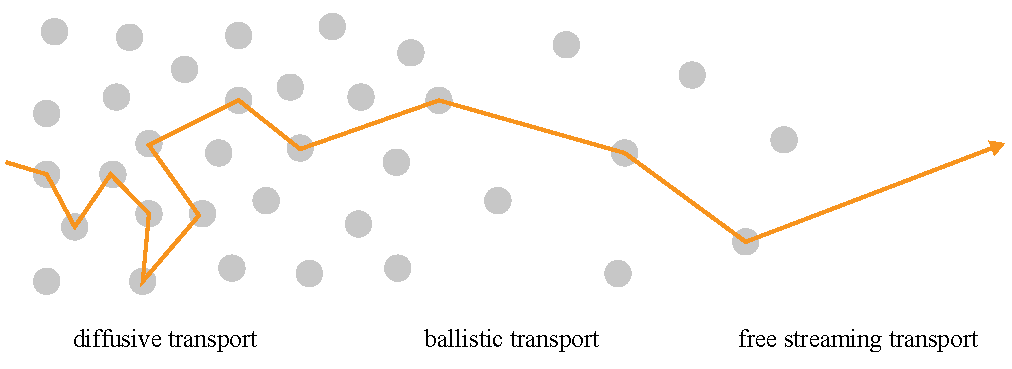
\includegraphics[width=0.9\textwidth]{06_fld/figures/fig_transport_regimes_mfp.pdf}
\caption{Intuition behind paramterizing the transport regime according to mean free path (average distance between two consecutive scattering events). Small mean free paths imply higher medium density, while larger mean free paths imply lower density or vacuum in case of infinity.}
\label{fig:fld_transport_regimes_mfp}
\end{figure}



The second factor in equation~\ref{eq:flux_limit_factors} is the ratio between the length of the flux-vector (according to diffusion) and the zero moment. If the magnitude of the flux-vector is small, while the total power $\phi$ is large, the incoming radiance is distributed equally over solid angle, which means that light is coming uniformly from all directions. If the flux-vector magnitude is large in comparison to the total power, the energy is concentrating in certain directions. In the extreme case, when the total power is equal to the flux-vector magnitude, the light comes only from a single direction.
\begin{figure}[h]
\centering
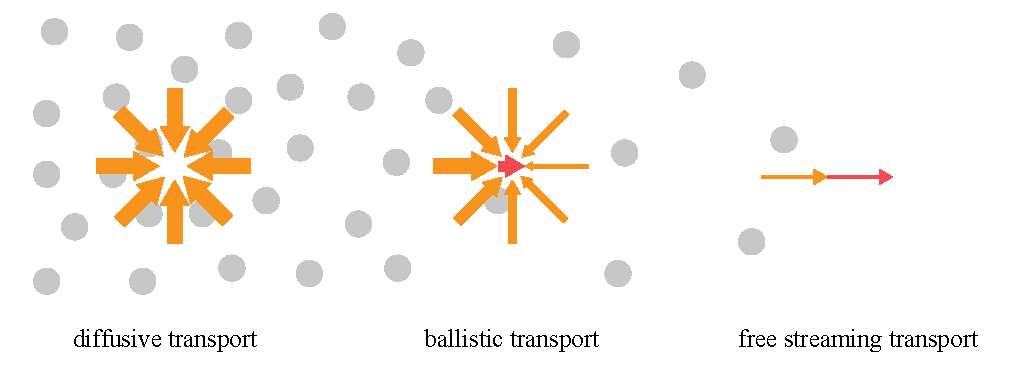
\includegraphics[width=0.9\textwidth]{06_fld/figures/fig_transport_regimes_moment_ratio.pdf}
\caption{Intuition behind paramterizing the transport regime according to the ratio between the total amount of light arriving at a point and the directionality given by the magnitude of the flux vector (red in the figure). A small ratio results from small directionality in relation to large amounts of light arriving. This implies a uniform distribution of light coming from all directions, which is the case for diffusive transport. The ballistic transport regime is characterized by increased directionality in relation to the amount of light. In free streaming transport, the magnitude of the flux vector equals the amount of light arriving. This is the case when light comes from a single direction.}
\label{fig:fld_transport_regimes_mfp}
\end{figure}

The two factors in equation~\ref{eq:flux_limit_factors} parameterize the transport regime according to the medium and the distribution of incoming light over solid angle respectively. Combined, they are a local measure for the transport regime in general (as perceived by diffusion). If the medium is very dense (small mean free path) and light arrives equally distributed from all directions (small moment ratio), diffusive transport is dominating and the flux-limit is not violated. The diffusion approximation is a good approximation in these scenarios. If the medium is very thin (large mean free path) and the moment ratio approaches one, we have ballistic transport. In the case of vacuum, when the moment ration is exactly one, we have the free streaming limit or vacuum, where light travels infinte distances unhindered.

The $1/3$ factor in equation~\ref{eq:flux_limit_factors} is ignored and $R$ is introduced, a transport measure according to the diffusion approximation:
\begin{align}
\label{eq:fld_transport_measure_R}
R\left(\vec{x}\right)
= 
\frac{\norm{\nabla\phi\left(\vec{x}\right)}}{\sigma_t\left(\vec{x}\right)\phi\left(\vec{x}\right)}
\qquad
\qquad
\begin{array}{cc}
R\left(\vec{x}\right)\rightarrow 0 : \text{diffussive transport}\\
R\left(\vec{x}\right)\rightarrow 1 : \text{streaming transport}
\end{array}
\end{align}
In section~\ref{sec:moment_closure}, the diffusion approximation was derived by assuming isotropic distribution of radiance and therefore the same requirement in the fux-limit contraint is seen where a small moment ratio is required and implies that light is arriving equally from all directions.

The idea of flux-limited diffusion is to avoid violation of the fux-limit and consquently prevent unphysical transport. The key idea behind flux-limited diffusion is to not only assume isotropic distribution, but also allow streaming transport and use the measure $R$, to locally realize the right mix between diffusive and streaming transport. The next important building block is therefore the question of how the diffusion equation looks like in the presence of streaming transport. This is outlined in the next section. Section~\ref{sec:fld_vef} will then develop flux-limited diffusion as a combination with classical diffusion.
